\documentclass[11pt]{article}
\renewcommand{\baselinestretch}{1.05}
\usepackage{amsmath,amsthm,verbatim,amssymb,amsfonts,amscd, graphicx}
\usepackage{blindtext}

\usepackage{caption}
\usepackage{enumitem}

%Additional Packages
\usepackage{enumitem}
\usepackage{graphics}
\usepackage{float}
\graphicspath{ {images/} }
%\usepackage[framed]{mcode}
\usepackage{hyperref}
\hypersetup{
	colorlinks=true,
	linkcolor=blue,
	filecolor=magenta,      
	urlcolor=cyan,
}

\topmargin0.0cm
\headheight0.0cm
\headsep0.0cm
\oddsidemargin0.0cm
\textheight23.0cm
\textwidth16.5cm
\footskip1.0cm
\theoremstyle{plain}
\newtheorem{theorem}{Theorem}
\newtheorem{corollary}{Corollary}
\newtheorem{lemma}{Lemma}
\newtheorem{proposition}{Proposition}
\newtheorem*{surfacecor}{Corollary 1}
\newtheorem{conjecture}{Conjecture} 
\newtheorem{question}{Question} 
\theoremstyle{definition}
\newtheorem{definition}{Definition}

\usepackage{indentfirst}
%\renewcommand{\thesubsubsection}{\thesubsection.\alph{subsection}}

\newcommand{\floor}[1]{\lfloor #1 \rfloor}

%SETUP PSUEDOCODE
\usepackage{tcolorbox}


%SETUP AtxMEGA128A1U
\usepackage{listings}

\usepackage{xcolor}
\definecolor{bluekeywords}{rgb}{0.13,0.13,1}
\definecolor{greencomments}{rgb}{0,0.5,0}
\definecolor{turqusnumbers}{rgb}{0.17,0.57,0.69}
\definecolor{redstrings}{rgb}{0.5,0,0}


%Set up code
\usepackage{listings}
\usepackage{color}

\definecolor{dkgreen}{rgb}{0,0.6,0}
\definecolor{gray}{rgb}{0.5,0.5,0.5}
\definecolor{mauve}{rgb}{0.58,0,0.82}

\lstset{frame=tb,
	language=C,
	aboveskip=3mm,
	belowskip=3mm,
	showstringspaces=true,
	columns=flexible,
	basicstyle={\small\ttfamily},
	numbers=none,
	numberstyle=\tiny\color{gray},
	keywordstyle=\color{blue},
	commentstyle=\color{dkgreen},
	stringstyle=\color{mauve},
	breaklines=true,
	breakatwhitespace=true,
	tabsize=3
}

%
% START OF DOCUMENT
%
\begin{document}
\captionsetup[figure]{labelfont=bf} 

\title{Lab 6}
\author{\textbf{Michael Arboleda}\\Lab Section: 7F34}
\maketitle
%
% PRELAB QUESTIONS
%
\section*{b. Answers to all pre-lab questions}



\begin{enumerate}[label={\arabic*)},font={\color{red}\bfseries}]
	%
	%1
	%
	\item What is the highest speed of communication the IMU
	can handle?
	\\[0.8ex]
	\textbf{ANS: } The highest speed of communication the IMU can handle is 10MHz
	%
	%2
	%
	\item In which order should you transmit data to the LSM330? LSB first or MSB first?
	\\[0.8ex]
	\textbf{ANS: } Data for the LSM330 should be transmitted with MSB first
	%
	%3
	%
	\item When using SPI, why do we have to write data in order to be able to read data? 
	\\[0.8ex]
	\textbf{ANS: } Since SPI is synchronous and transmits bi-directionally, the master must transmit data so data from the slave can be acquired.
	%
	%4
	%
	\item How are the accelerometer and gyroscope enabled?
	\\[0.8ex]
	\textbf{ANS: } The accelerometer is enabled by setting $\overline{SSA}$ to be true and SEN\textunderscore SEL to 1. The gyroscope is enabled by setting $\overline{SSG}$ to be true and SEN\textunderscore SEL to 0.
	%
	%5
	%
	\item Why is it a good idea to modify global flag variables inside ISRs instead of doing everything inside of them?
	\\[0.8ex]
	\textbf{ANS: } It is a good idea to not do everything inside an ISR because ISR stops processes that are running normally. Thus it is good to have the least amount of code/operation inside an ISR so that the program can continue to execute normally
\end{enumerate}
%
% PROBLEMS ENCOUNTERED
%
\section*{c. Problems Encountered} 
Problems encounter was that the wrong data was being outputted. This is because in the LSM\textunderscore READ, the return statement returned spi\textunderscore read, but this happens after the selects for both the accelerometer or gyroscope are off, so it was never actually reading data from the LSM
%
% FUTURE WORK
%
\section*{d. Future Work/Applications}
Future application would be using the LED with accelerometer. This could be change the color once a certain value with the accelerometer is reach. This could then be used for devices that are remote controlled.  
%
% SCHEMATICS
%
\section*{e. Schematics}
N/A
%
% PSEUDOCODE
%
\newpage
\section*{g. Pseudocode/Flowcharts}
%
% PSEUDOCODE PART A
%
\textbf{\textcolor{blue}{Pseudocode for Lab6b.c:}}
\begin{tcolorbox}
\begin{verbatim}
MAIN:
    * Call Change_CLK_32HZ Function
    * Call spi_init Function
    
    WHILE(TRUE){
        spiWrite(0x53)
    } 
END  

FUNCTION spi_init 
    * Set up port F
    * Set up port A
    * Set up SPI ctrl
    
FUNCTION spiWrite
    * Write to DATA reg
    
    WHILE(IF flag not set){}
    
    * Return data in SPIF.DATA
    
FUNCTION spiRead
    * return spiWrite(0xFF)
        
FUNCTION Change_CLK_32HZ
    * Enable the new oscillator

    WHILE(OSC FLAG not set){}

    * Write the “IOREG” signature to the CPU_CCP reg
    * Select the new clock source in the CLK_CTRL reg  
\end{verbatim}
\end{tcolorbox}
%
% PSEUDOCODE PART F
%
\newpage
\textbf{\textcolor{blue}{Pseudocode for Lab6f.c:}}
\begin{tcolorbox}
\begin{verbatim}
MAIN:
    * Call Change_CLK_32HZ Function
    * Call spi_init Function
    * Call USART_INIT Function
    * Call spi_init Function
    * Call accel_init Function
    * Call gyro_init Function
    * Set up interrupts
    * Clear data in Gyro
    
    WHILE(TRUE){
        IF(accelerometer data is ready){
            * Call READ_DATA_ACCEL() Function
        }
        IF(gyro data is ready){
            * Call READ_DATA_GYRO() Function
        }
    }
    
END

FUNCTION LSM_READ
    IF(GYRO selected){
        * Select/Enable Gyro
    }
    IF(ACCEL selected){
        * Select/Enable ACCEL
    }
    
    * write adrres
    * save data at address
    
    IF(GYRO selected){
        * disable Gyro
    }
    IF(ACCEL selected){
         * disable ACCEL
    }
    
    * return saved data    
\end{verbatim}
\end{tcolorbox}




\begin{tcolorbox}
\begin{verbatim}    
FUNCTION LSM_WRITE
    IF(GYRO selected){
        * Select/Enable Gyro
    }
    IF(ACCEL selected){
        * Select/Enable ACCEL
    }
    
    * write adrres
    * write data
    
    IF(GYRO selected){
        * disable Gyro
    }
    IF(ACCEL selected){
        * disable ACCEL
    }
    
FUNCTION accel_init
    * Set up PORT C interrupt
    * route the DRDY signal to INT1_A and enable
      INT1 with a rising edge (active high)
    * configure the accelerometer to have the highest
      possible output data rate as well as enable the X, Y,
      and Z axes.  
 
FUNCTION gyro_init
    * Set up PORT A interrupt
    * GYRO_ENABLE bit on PORTA     
    * configure the gyroscope to have the highest possible
      output data rate as well as enable the X, Y, and Z axes.
    * Set the I2_DRDY bit
    * Choose 2000 dps for the full-scale selection bits
  
ISR(PORTA_INT0_vect)
    * Preserve Status reg
    * Set int flags
    * Set global var flag
    * Restore Status reg  

ISR(PORTC_INT0_vect)
    * Preserve Status reg
    * Set int flags
    * Set global var flag
    * Restore Status reg
\end{verbatim}
\end{tcolorbox}




\begin{tcolorbox}
\begin{verbatim}
FUNCTION DISPLAY_GYROACCEL_INFO
    * Transmit start byte 
    * OUT CHAR ACCEL DATA
    * OUT_CHAR GYR0 DATA
    * Transmit end byte
    
FUNCTION READ_DATA_ACCEL
    * Read accel data
    * Reset accel global flag

FUNCTION READ_DATA_GYRO
    * Read gyro data
    * Reset gyro global flag    

FUNCTION CLR_GYRO
    * STORE GYRO info
    
FUNCTION USART_INIT
    * Set port D for USART com
    * Set up Ctrl B and C
    * Set up baud rate    

FUNCTION OUT_CHAR
    While(Transmitting){}
    * Return USART Data in a CHAR

FUNCTION spi_init 
    * Set up port F
    * Set up port A
    * Set up SPI ctrl

FUNCTION spiWrite
    * Write to DATA reg

    WHILE(IF flag not set){}

    * Return data in SPIF.DATA
\end{verbatim}
\end{tcolorbox}




\begin{tcolorbox}
\begin{verbatim}
FUNCTION spiRead
    * return spiWrite(0xFF)

FUNCTION Change_CLK_32HZ
    * Enable the new oscillator

    WHILE(OSC FLAG not set){}

    * Write the “IOREG” signature to the CPU_CCP reg
    * Select the new clock source in the CLK_CTRL reg

\end{verbatim}
\end{tcolorbox}


    












\newpage
%
%
% PROGRAM CODE
%
%
\section*{h. Program Code}
\textbf{\textcolor{blue}{Code for Lab6b.c:}}
\lstinputlisting{Lab6b.c}
\newpage
\textbf{\textcolor{blue}{Code for Lab6f.c}}
\lstinputlisting{Lab6f.c}
\newpage
%
%
% APPENDIX
%
%
\section*{i. Appendix}
\begin{figure}[H]
	\centering
	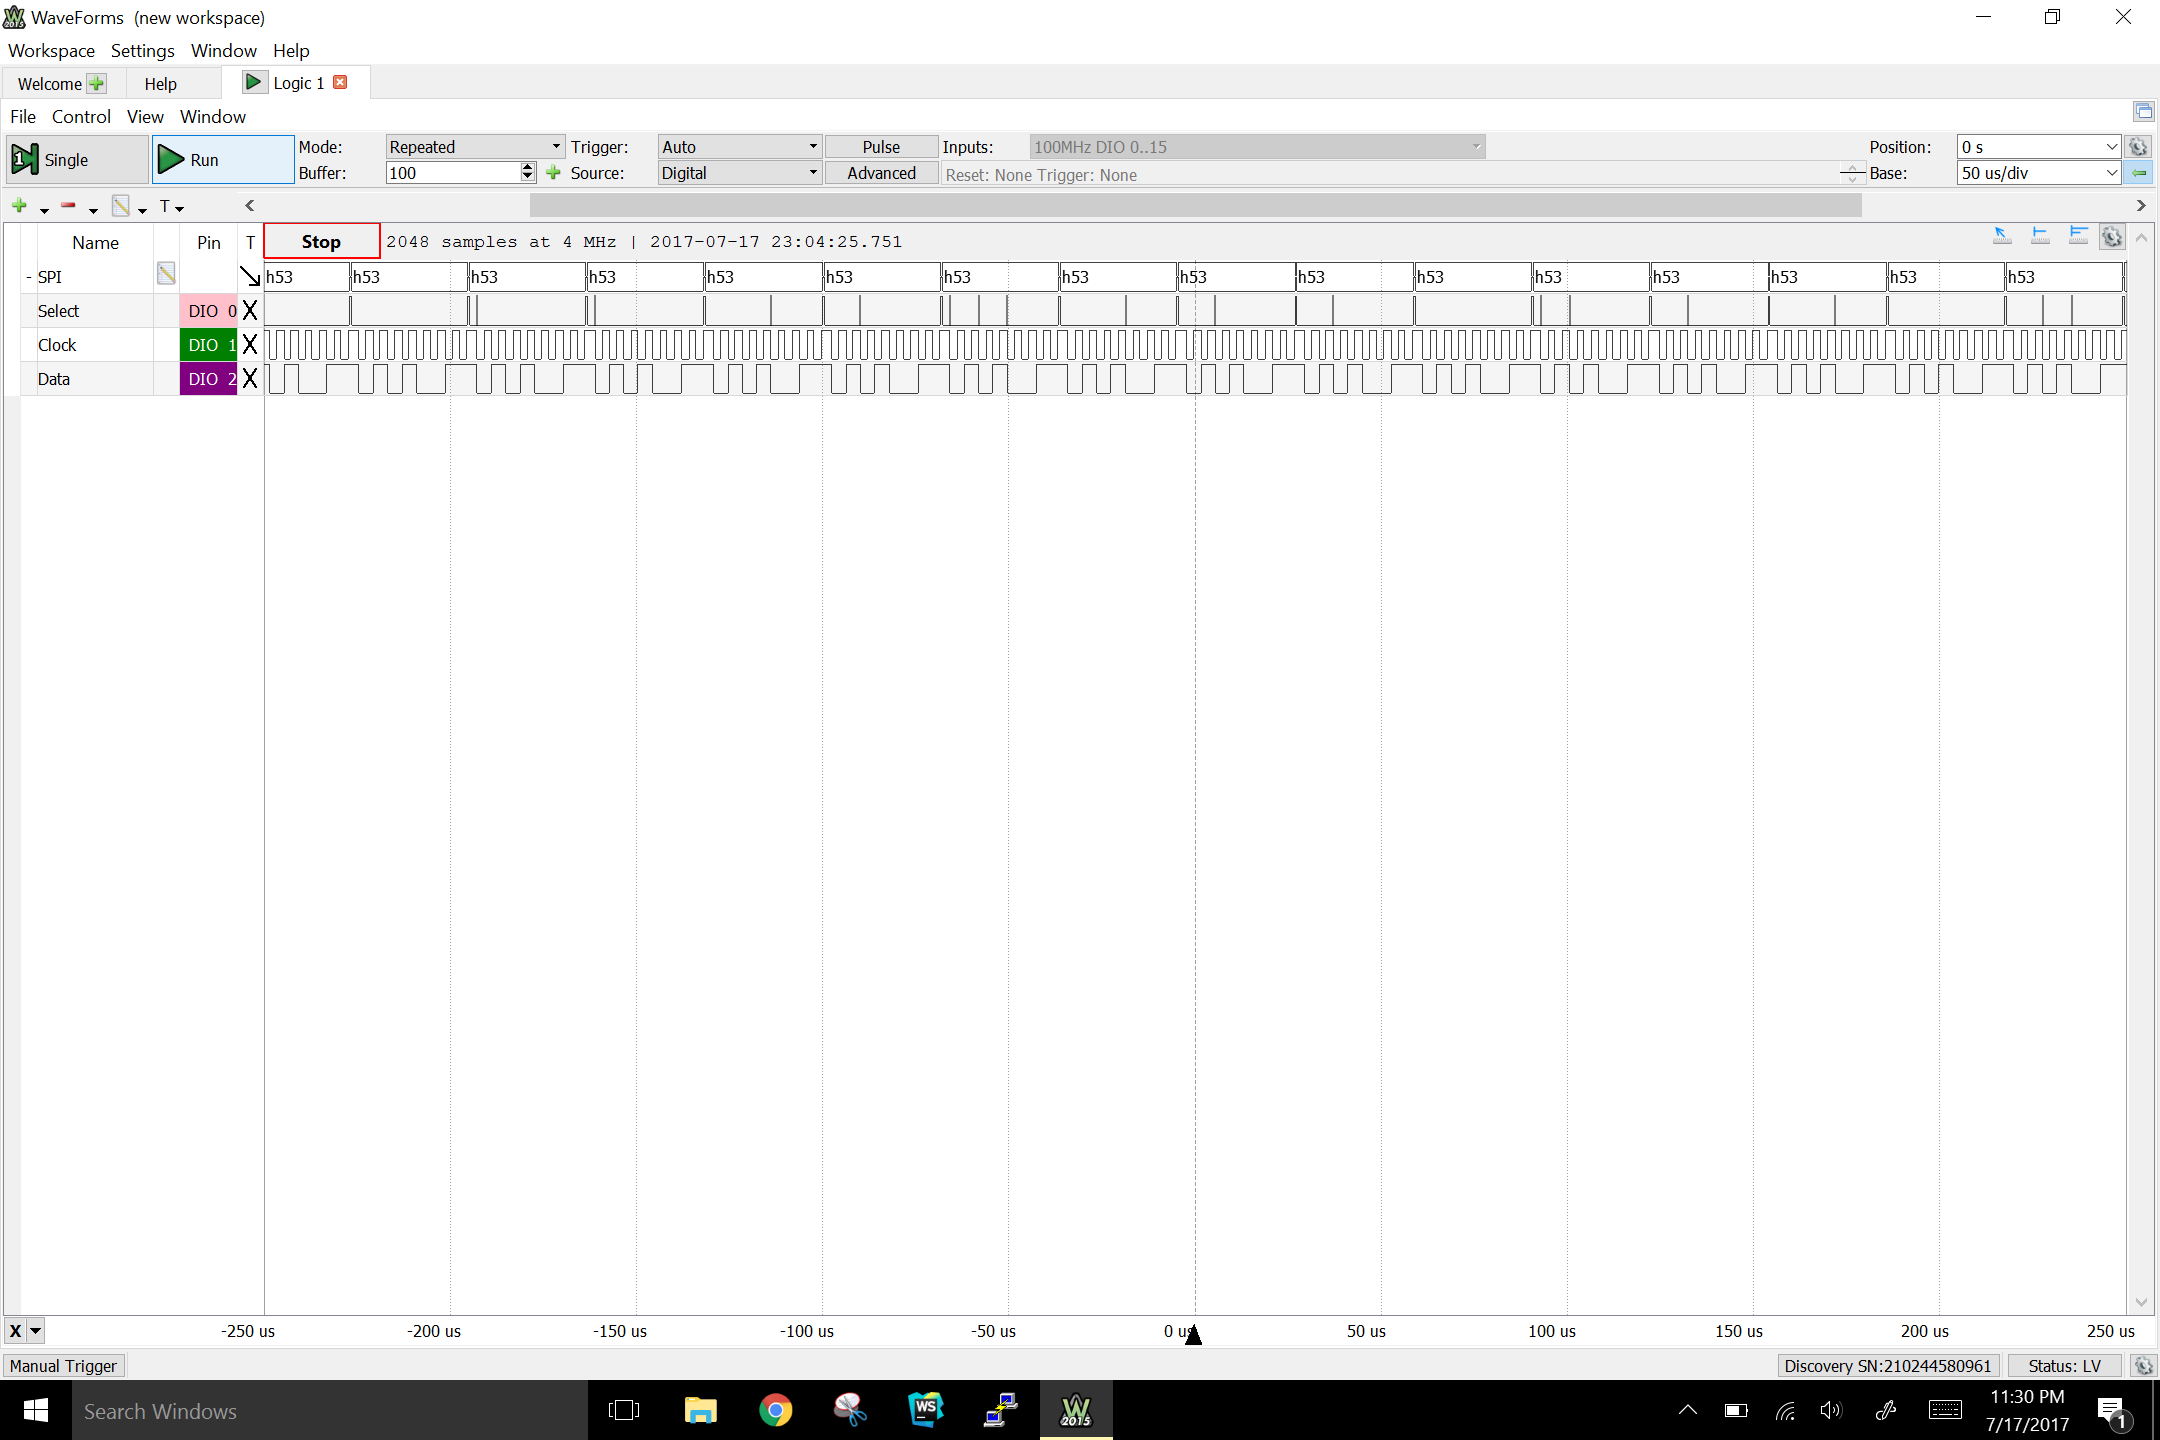
\includegraphics[width=\textwidth]{dad}
	\label{fig:a}
	\caption{DAD reading of SPI}
\end{figure}
\begin{figure}[H]
	\centering
	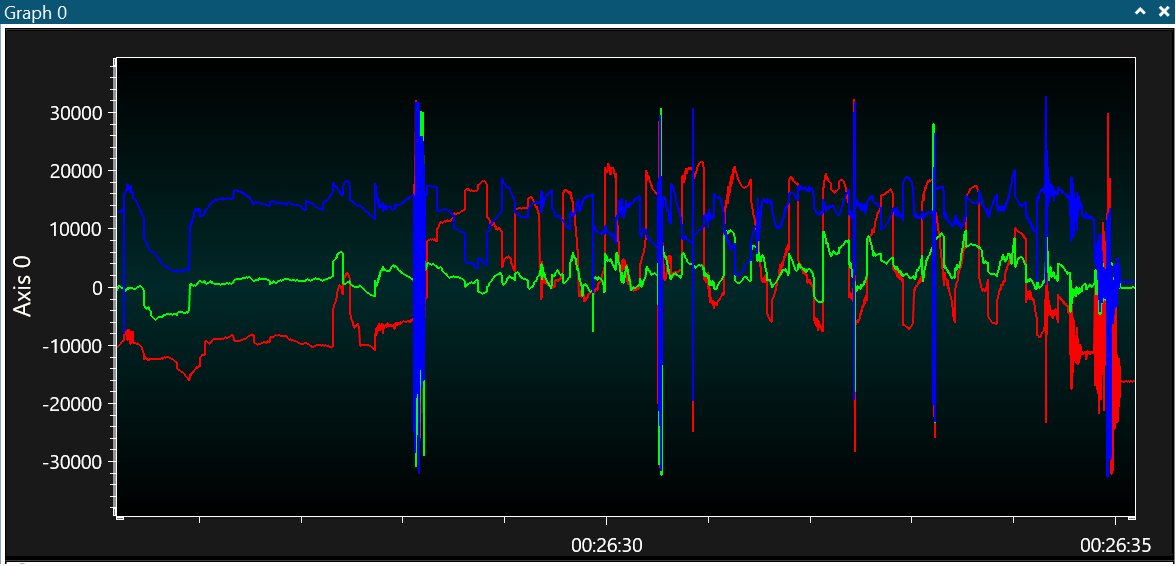
\includegraphics[width=\textwidth]{accel}
	\label{fig:b}
	\caption{Graph of accelerometer data}
\end{figure}
\begin{figure}[H]
	\centering
	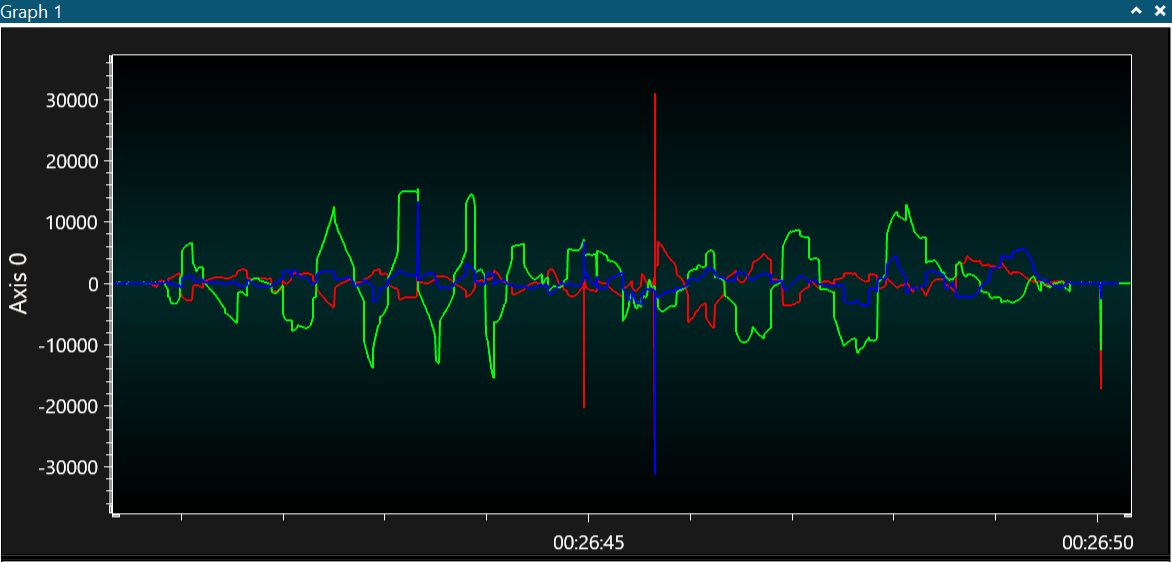
\includegraphics[width=\textwidth]{gyro}
	\label{fig:c}
	\caption{Graph of gyroscope data}
\end{figure}
%
% HEADER FILES
%
\newpage
%
% Clk_32Mhz
%
\textbf{\textcolor{blue}{Code for Clk\textunderscore 32MHz.h:}}
\lstinputlisting{Clk_32MHz.h}
\newpage
\textbf{\textcolor{blue}{Code for Clk\textunderscore 32MHz.c:}}
\lstinputlisting{Clk_32MHz.c}
%
% LSM
%
\newpage
\textbf{\textcolor{blue}{Code for LSM.h:}}
\lstinputlisting{LSM.h}
\newpage
\textbf{\textcolor{blue}{Code for LSM.c:}}
\lstinputlisting{LSM.c}
%
% SPI
%
\newpage
\textbf{\textcolor{blue}{Code for SPI.h:}}
\lstinputlisting{SPI.h}
\newpage
\textbf{\textcolor{blue}{Code for SPI.c:}}
\lstinputlisting{SPI.c}
%
% USART 
%
\newpage
\textbf{\textcolor{blue}{Code for USART.h:}}
\lstinputlisting{USART.h}
\newpage
\textbf{\textcolor{blue}{Code for USART.c:}}
\lstinputlisting{USART.c}
%
%
%
\newpage
\textbf{\textcolor{blue}{Code for constants.h:}}
\lstinputlisting{constants.h}
\end{document}